
\documentclass[11pt]{report}
\usepackage{graphicx}
\usepackage{url}
\usepackage{amsmath}
\usepackage{verbatim}
\title{TDT4255 Assignment 3}
\author{Knut Halvor Skrede \& Ole Magnus Ruud}
\begin{document}
\maketitle
\clearpage


\section*{Abstract/Summary}
        
% Lab-report presents documentation of your work which was done during the exercise. 
% It is important
% that the reader can understand what the group has done and how it came to the solution.
% In short, abstract should contain overview of:
% – what the task of the exercise was
% – how it was solved
% – what works
% – what does not work
% – if something extra was done by the group
% – if something should have been done in another way

The task was to implement a simple multicycle CPU. A top level architecture 
was proposed in the assignment text, we chose to implement the CPU in this way. 
We could use the ALU we made from the previous assignment, but we chose to use
the one included in the support files. The CPU should load instructions into 
memory and execute them. A program counter will be used to walk through the 
instructions. A BNZ (branch if not zero) instruction can also be used, this 
instruction will load the program counter with a given address if the zero flag
in the status register is not set. Additionally the CPU should implement a 
LDI (load immediate) instruction that loads the the register with a value. 
The cpu should also implement the ALU functionality.

We chose to use the instruction word layout proposed in the assignment text.

The control unit implements a simple fetch-execute state machine.

The assignment was also to write a simple program to run on the CPU, 
we chose to implement fibonacci.

\section*{Introduction}

% Present what the task within the exercise is and what challenges it
% gives.  For example, which kind of program has to be written and
% which hardware has to be used.  Short introduction to how the group
% has solved this task.  It is important that what has been
% accomplished is clearly presented.  If there is something in the
% exercise what has not been completed or what does not function as it
% should, it should also be described.  If applicable, write on the
% motivation and solution(s) for extra functionality which the group
% has set in.

The task of this assignment was to expand the design from the previous
assignment with pipelining and a data storage memory, and make it work
on Nalle. To do this, it
was necessary to add registers between each pipelining stage containing
all information and control signals needed for later stages. It was also
necessary to take dependancy hazards into account by writing back results
to where it is needed in the earlier pipelining stages. 

We used the suggested solution as a starting point. %Meeeeeeer!

\section*{Suggested Solution}

% Present concisely an outline of how the task was solved.  This is
% the place to write in greater detail about how the group was
% developing ideas for achieving solution.  Add an outline of, for
% example, how hardware is built up and how it functions.  It is
% advised to use concise and clear flow diagrams, UML or block
% diagram.  All code should be delivered in a separate file. It is
% important that documentation contains enough description of the
% program so that the reader can understand how the program works and
% what files with the source code are attached. Write about how the
% group has come to the solution, what tests were used to ensure that
% the program runs as it should, for example, what documentation the
% group has used, possibly some additional sources which were helpful
% to do the exercise.  Remember that documentation is a part of the
% grade. So, it is not enough to have a brilliant solution if the
% reader can't understand how it is meant to work.

\subsection*{Design}

% Write somthing about instruction format, implemented functions. Data sizes and so on.
% Describe computation flow, what happens at each stage
\subsubsection*{Instruction format}
As our instruction format we decided to use a slightly modified version of the
suggested format from assignment 2, shown in figure 1.

\begin{table}[h]
  \centering
  \begin{tabular}{|l|l|l|l|l|l|l|l|}
    \hline
    Name: 		&	Opcode		&	unused	&	funct	&	Imm		&	Rd		&	Ra	&	Rb	\\\hline
    Bits: 		&	31-29		&	28-24	&	23-20	&	19-12	&	11-8	&	7-4	&	3-0	\\\hline
  \end{tabular}
  \caption{Instruction set format}
\end{table}

 \begin{itemize}
\item Opcode: used to determine the control signals in the cpu given different instructions.	
\item Funct: used for choosing the ALU instruction.
\item Immediate: used for Load Immediate, load the register with the given value and for branch instruction to set the new value in the programme counter
\item Rd : number of the register which will be written
\item Ra : number of register A
\item Rb : number of register B
\end{itemize}

\begin{table}[h]
  \centering
  \begin{tabular}{|l|l|l|}
    \hline
    Name&Opcode&Comment \\
    \hline
    ALU\_INST	&001	&Writes alu result to register\\
    BNZ			&011	&Loads pc register if zero flag is set\\
    LDI			&010	&Loads register with value\\
    LOAD		&110	&Writes register Ra to memory at address given by immediate\\
    STORE		&100	&Loads register Rd with memory at address given by immediate\\
    \hline
  \end{tabular}
  \caption{Instruction set for the ALU, not including the alu functionality}
\end{table}

\begin{table}[h]
  \centering
  \begin{tabular}{|l|l|l|}
    \hline
    Name&Funct&Comment \\
    \hline
    MOVE	&0000	& sets output of ALU out to input A\\
    AND		&0001	& Bitwise AND\\
    ADD		&0111	& Arithmetic ADD\\
    \hline
  \end{tabular}
  \caption{Function set for the ALU}
\end{table}


\subsubsection*{Implemented functions}
\subsubsection*{Instruction flow}
We will here describe the basic flow of operations for an instruction
through our processor architecture stage by stage without hazards handling.
\begin{description}

\item[Instruction fetch]

Instructions starts out by being fetched based on the program counter from the
instruction memory to the IF/ID register. This is the complete basic operation of the 
instruction fetch stage.
\item[Decode]

In the decode stage the most basic action is the forwarding of the Rd, Immediate and
the function field to the ID/EX register. The Ra and Rb fields are sent to the regfile, 
and the corresponding outputs are written to the ID/EX A and B field. 
The immediate field is also connected to the data memory read address, as this value
needs to be read on a rising edge because of the memory implementation.

Based on the opcode of the instruction, control has to write several control signals 
to the ID/EX register. These are divided into control signals for the Execute stage
and control signals for the writeback stage.

The execute control signals are memory write enable, which is set for memory write instructions,
and status write enable, which is set for ALU instructions.

The writeback control signals are source select and register write enable. 
The source select is the control signal for the register input selector,
which is set to alu output for alu operations, memory output 
for load instructions and immediate for load immediate. 
The register write enable is set for all instructions resulting in a register write.

\item[Execute]

In the execute stage the Rd, immediate and writeback control signal fields are 
forwarded from ID/EX to EX/WB. 

The ALU combinatorially computes an output value based on
the A, B and function fields of the ID/EX register, and stores it in an ALU field in
the EX/WB register. The output from the ALU status is sent to the Status register along
with the status register write signal from the ID/EX register which decides if the 
register is written.

The immediate value from the Decode stage has now been caught 
by the Data memory, and the value stored at this address is written to the memory field
of the EX/WB register. The immediate, A and memory write enable fields of the ID/EX register
are sent to the write address, write data and write enable inputs of the data memory,
respectively. If the write enable is asserted, the data is written.

\item[Writeback]

In the writeback stage the register file is written if the register write enable
signal of the EX/WB register is asserted. The value written is selected with a register
input mux based on the source select signal in the EX/WB register with all the data fields
of EX/WB as inputs. The register destination is decided by the propagated Rd field of the
EX/WB register.

\end{description}

\subsubsection{Hazards handling}

A big part of this assignment was the Hazards handling

\subsection*{Approach}

%We started by making skeleton modules for all the components, mapping
%the signals between them. After that we implemented the simplest
%components. To make sure nothing was wrong before writing the more
%difficult components, we wrote simple testbenches for them. We then
%proceeded to implement the control unit, which we considered to be the
%most challenging component. We then wrote a more general testbench for
%the CPU, and after debugging and figuring out some timing issues, we
%tested it on nalle running a program calculating fibonacci numbers.

Our approach to the problem in this excercise was to construct all the 
modules described in the architecture diagram, starting with the simplest.  %DIAGRAM!
This included the writeback muxes between the register file and the id/ex
pipeline register, and the writeback muxes between the id/ex pipeline 
register and the ALU and data memory as we felt confident we were going 
to get the hazards handling working. 
Some of the modules like the program counter and status register 
we reused from the previous assignments.

When the muxes were finished, we had a good indication on what control
signals would be needed for all the pipelining stages, and so we could 
implement the pipelining registers with all of these control signals.

The final and most difficult component we implemented was the control
module setting all the control signals. When we thought we had it right
everything was sewed together and we could test it with a testbench
from the previous assignment. After some debugging in Modelsim we had 
a working architecture.

\subsection*{Implementation}

Our implementation consists of the following components
ordered by their appearance in the pipelining stages:
	
\begin{enumerate}
\item Program counter.
\item Instruction memory.
\item IF/ID pipeline register.
\item Control unit.
\item Register file.
\item Register to ID/EX muxes.
\item ID/EX pipeline register.
\item ID/EX to ALU and data memory muxes.
\item ALU.
\item Status Register
\item Data memory.
\item EX/WB pipeline register.
\item Register input mux.
\end{enumerate}
	
We will now describe the components.
\subsubsection*{Program Counter}
%The program counter is initiated to 0 on reset and is updated every control cycle
%with either an increment or an immediate value from the instruction. 
%We discussed using a relative jump instead of just loading a value, 
%but decided to drop this as there is no need for relative jumps when running 
%single programs and we have full control of memory.
The program counter is the same one used in the previous assignment. 
It is a counter with an initial value of 0 after reset, with a built in
mux choosing between a provided immediate value, and the incrementation of
the current value. It also takes in a write enable that is not needed in
the current architecture, but that would be if we decided to expand the 
instruction set in the future.

\subsubsection*{Instruction memory}
The instruction memory is an instantiation of the provided memory component taking in
output from the program counter and providing the instruction at the provided
address.
\subsubsection*{IF/ID pipeline register}
Since the instruction is stored on the output register of the instruction memory,
the IF/ID pipeline register component is actually just an abstraction of this, sending 
most of its input straight through, and only registering the valid bit, provided by
the control module.

\subsubsection*{Control Unit}

The control unit is the most complex component in our design, as all the control
signals in the decode stage is set here, as well as the future control signals for
the execute and writeback stage that must be written to the ID/EX pipeline register.
The component is purely combinatorial, with outputs based on the current instruction in the
IF/ID register and some fields in the other pipeline registers to handle hazards as
described in the design section. %OBS!

\subsubsection*{Register file}
The register file is an instantiation of the delivered register file, with 
2 combinatorial read adresses with corresponding outputs, and one sequential
write address and data port.

\subsubsection*{Register to ID/EX muxes}
Based on two control signals from the control unit, this double mux combinatorially
decides the input of the two operand fields of the ID/EX register. It can 
either be from the register or the writeback signal from the writeback stage.
\subsubsection*{ID/EX pipeline register}
This is a simple sequentially written register. The contents are described in the 
design section. %OBS!! Make it so!
\subsubsection*{ID/EX to ALU and data memory muxes}
This component works the same way as the Register to ID/EX mux, but the source of the 
mux control signals is the ex field of the ID/EX register, and the ouput is connected
to the ALU and Data memory data input.

\subsubsection*{ALU}
The alu is the simple handed out component.
\subsubsection*{Status Register}
We use our Status Register implementation from the previous assignment, but have
built in the writeback mux to be controlled by the write status register signal.
When the status write signal is asserted, the mux will also choose the current 
status signal from the ALU, even before it is written to the register.
\subsubsection*{Data Memory}
As with the Instruction memory, this is an instantiation of the handed out memory
module, only used for data. This implies an 8-bit width. Because it needs the read address
on the rising edge, we had to connect the read address port to the immediate value of the
if/id register.
\subsubsection*{EX/WB pipeline register}
As with ID/EX this is just a simple register. Fields are described in the design section.
\subsubsection*{Register input mux}
Our last component is the muxer choosing what value of the EX/WB register to send to the
register file. 
%The status register is just a register with a write enable, and the register 
%multiplexer is just a mux placed in a component to clean up our CPU code.  


\begin{table}[h]
  \centering
  \begin{tabular}{|c|c|c|}
    \hline
    Name&Opcode&Comment \\
    \hline
    ALU\_INST&000&Writes alu result to register\\
    BNZ&001&Loads pc register if zero flag is set\\
    LDI&010&Loads register with value\\
    \hline
  \end{tabular}
  \caption{Instruction set for the cpu, not including the alu functionality}
\end{table}

\subsection*{Testing}

For testing we wrote the following programs:

\subsubsection*{Instruction flush test}

This program tests if the instruction after a branch is successfully flushed.
The program segment loads two values, 246 and 1. It then adds 1 to 246 and
branches back to the add instruction until it reaches 255 and then overflows
to 0. After the overflow add the branch should not be taken and the next instruction
should be executed. If it fails, the register holding 1 will be loaded with 10
and the program will net perform as expected.

\begin{table}[h]
  \centering
  \begin{tabular}{|c|c|c|c|c|c|c|}
    \hline
    Line Nr &	Opcode		&	funct	&	Imm	&	Rd	&	Ra	&	Rb	\\\hline
    	0	&	LDI			&			&	246	&	1	&		&		\\\hline
    	1	&	LDI			&			&	1	&	2	&		&		\\\hline
    	2	&	ALU\_INST	&	ADD		&		&	1	&	2	&	1	\\\hline
    	3	&	BNZ			&			&	2	&		&		&		\\\hline
    	4	&	LDI			&			&	10	&	2	&		&		\\\hline
  \end{tabular}
  \caption{Program to test branching}
\end{table}

\begin{figure}
\centering
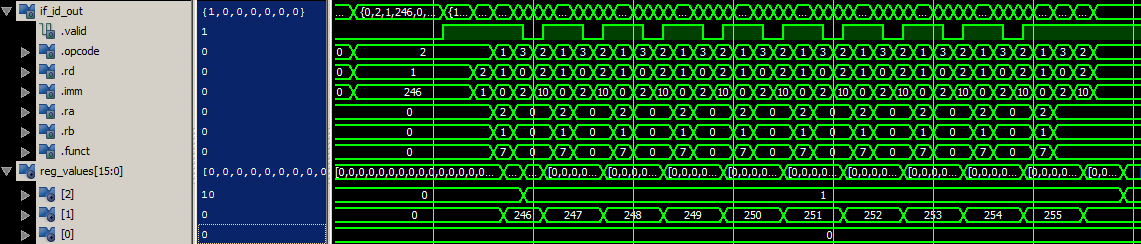
\includegraphics[width=.95\linewidth]{test1.png} \\
\caption{This figure shows the waveform from the testbench, 
most of the register signals has been removed, this is because they are not beeing used.}
\end{figure}


\subsubsection*{Datadependency test}

This program test if the dataforwarding is successfull.

\begin{table}[h]
  \centering
  \begin{tabular}{|c|c|c|c|c|c|c|}
    \hline
    Line Nr &	Opcode		&	funct	&	Imm	&	Rd	&	Ra	&	Rb	\\\hline
    	0	&	LDI			&			&	18	&	1	&		&		\\\hline
    	1	&	LDI			&			&	2	&	2	&		&		\\\hline
	\multicolumn{7}{|c|}{Test 1: Dataforwarding from writeback- to execute-stage (one-stage forwarding)}\\\hline
    	2	&	ALU\_INST	&	ADD		&		&	1	&	2	&	1	\\\hline
    	3	&	ALU\_INST	&	ADD		&		&	1	&	2	&	1	\\\hline
    	4	&	ALU\_INST	&	ADD		&		&	1	&	2	&	1	\\\hline
	\multicolumn{7}{|c|}{Test 2: Dataforwarding from writeback- to decode-stage (two-stage forwarding)}\\\hline
    	5	&	ALU\_INST	&	ADD		&		&	1	&	2	&	1	\\\hline
    	6	&	ALU\_INST	&	ADD		&		&	1	&	2	&	2	\\\hline
    	7	&	ALU\_INST	&	ADD		&		&	1	&	2	&	1	\\\hline
  \end{tabular}
  \caption{Program to test data forwarding}
\end{table}

\begin{figure}
\centering
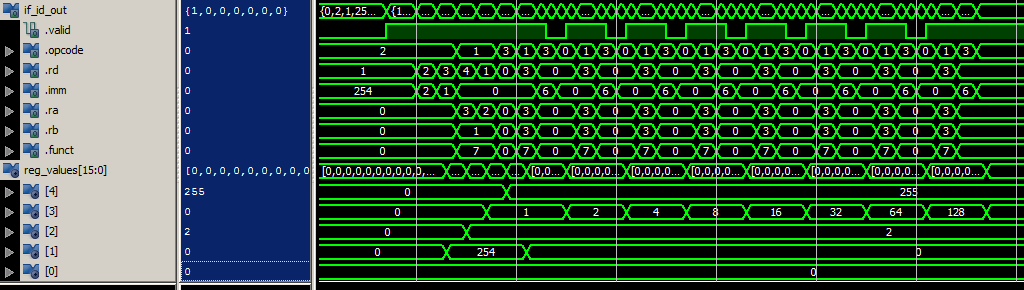
\includegraphics[width=.95\linewidth]{test3.png} \\
\caption{This figure shows the waveform from the testbench, 
most of the register signals has been removed, this is because they are not beeing used.}
\end{figure}

\subsubsection*{Status register test}

This program test if the statusregister is successfully forwarded.
It first loads 254 to register 1, 2 to register 2 and 1 to register 3.
It then adds 254 and 1 and writes it to register 4, the result should because
255. It then adds 2 to 254, this operations should overflow and result in zero,
resulting in the following branch instruction not to be taken. The instructions
following this test should count upwards in the power of 2 until it overflows
and stops. This test is located in file 'cpu\_testbench3.vhd'.

\begin{table}[h]
  \centering
  \begin{tabular}{|c|c|c|c|c|c|c|}
    \hline
    Line Nr &	Opcode		&	funct	&	Imm	&	Rd	&	Ra	&	Rb	\\\hline
    	0	&	LDI			&			&	254	&	1	&		&		\\\hline
    	1	&	LDI			&			&	2	&	2	&		&		\\\hline
    	2	&	LDI			&			&	1	&	3	&		&		\\\hline
    	3	&	ALU\_INST	&	ADD		&		&	4	&	3	&	1	\\\hline
    	4	&	ALU\_INST	&	ADD		&		&	1	&	2	&	1	\\\hline
    	5	&	BNZ			&			&	0	&		&		&		\\\hline
    	6	&	ALU\_INST	&	ADD		&		&	3	&	3	&	3	\\\hline
    	7	&	BNZ			&			&	6	&		&		&		\\\hline

		\end{tabular}
  \caption{Program to test data forwarding}
\end{table}

\begin{figure}
\centering
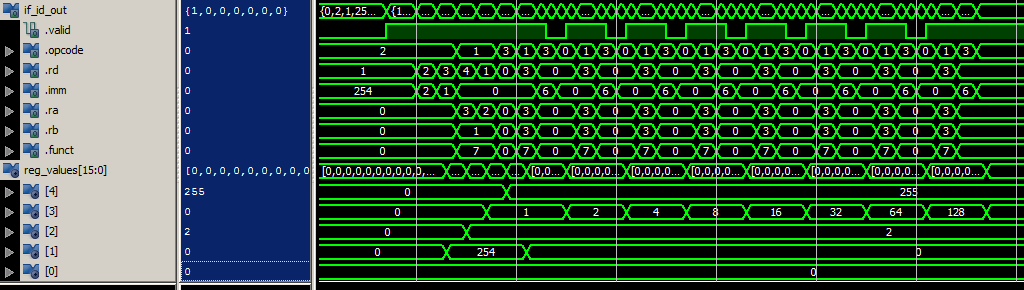
\includegraphics[width=.95\linewidth]{test3.png} \\
\caption{This figure shows the waveform from the testbench, 
most of the register signals has been removed, this is because they are not beeing used.}
\end{figure}


\subsection*{Synthesis}

From the synthesis report we see that
\begin{enumerate}
\item The regfile muxer inferred 8 1-bit multiplexers, this was a
  little strange as we expected 1 8-bit multiplexer.  This does not
  matter to the functionality though.
\item The sr module inferred one D-type flip flop, this is exatly what
  we wanted.
\item The pc module inferred one 8-bit counter, this is also exactly
  what we wanted.
\item The control module inferred 1 D-type flip flop, this is used to
  hold the current state (fetch or execute), the rest is
  combinatorial, so this is also what we wanted.
\item the toplevel and cpu modules did not infer anything, which was
  expected as they are simply mapping signals between the other
  modules.
\end{enumerate}

The estimated maximum clock frequency was 61.747MHz.

Selected Device : v1000efg860-6 

Usage of selected device:
\begin{table}[h]
  \centering
  \begin{tabular}{|l|l|l|} 
    \hline
    Number of Slices:&252 out of 12288&2\% \\ 
    Number of Slice Flip Flops:&205 out of 24576&0\% \\
    Number of 4 input LUTs:&454 out of 24576&1\% \\
    Number of bonded IOBs:&54 out of 664&8\% \\ 
    Number of BRAMs:&2 out of 16&12\% \\  
    Number of GCLKs:&2 out of 4&50\% \\
    \hline
  \end{tabular}
\end{table}


We got no errors from the place and route report, all constraints met,
and all signals routed.

\section*{Result}

% Present the result of the work. What works and what does not. 
% What the problems were if there were
% any. Or even better: what was fantastic in the group's work.
% Here is the place to add some screen-shots, debug outputs or similar to
% support the documentation. It is also the place to praise or show more
% critique towards the presented work.

Everything seemed to work after a couple of days work, 
both simulation and testing on nalle.

However, we had previously tried some different solutions
which did not work, and we realized that we did not understand why they did 
not work. We first tried to write to the registers on the rising edge of the clock, 
but this did not work. We then used the write enable signal as the clock 
on the registers and everything worked great.
However, we changed this later, when we discovered what we did wrong earlier,
which was having registers on the output of the control unit. After that
we removed the registers on the control unit and set the registers to be
written on the rising edge of the clock, and everything worked the way we
intended it to.

\section*{Evaluation}

% If there is something about the exercise what should be changed, 
% mention it here – text in the
% compendium, support files, exercise itself or something else which
% us as teaching staff should see to.

This assignment was very well defined compared to the previous. There was
alot less guesswork involved during the design process. We found this to
be more educational as we could focus on the tasks, in contrast to
making tasks up.

\section*{Conclusion}

% Round up - what works, what does not work. Comment on the exercise. 
% Write a bit about what was easy and what not so.

It was easy to map everything together and create most of the components. 
The difficult part of this assignment was to figure out the timing 
and syncronization, what signals to register and when they where 
ready to be read. All in all this was a fun and educational exercise.

\section*{References}

[1] http://en.wikipedia.org/wiki/Mealy\_machine

\end{document}


